\subsection{Effect of Noise}
\label{EffctOfNoise}

As mentioned in Sections \ref{OrdLstSqrRes} - \ref{BaysRes}, all three inversion methods perform well around the sand bar at $x \approx 900$ m but problems are noted as one moves sea-ward. This deviation between the approximated solution and the true solution is attributed to noise in the measured wave number profile; to see why, consider the difference between the calculated wave profile and the measured profile (Figure \ref{effectivewavenumbernoise}). As can be seen, the calculated wave number exhibits a smooth shape similar to the true bathymetry profile. Since we are using the same forward model to invert for the bathymetry we expect the calculated bathymetry to behave similarly to the measured wave number. At $x \approx 800$ m, Figure \ref{effectivewavenumbernoise} shows a distinct jump in the measured wave number which accounts for the mirrored behaviour in the real data results for all three methods.

\begin{figure}[H]
\center
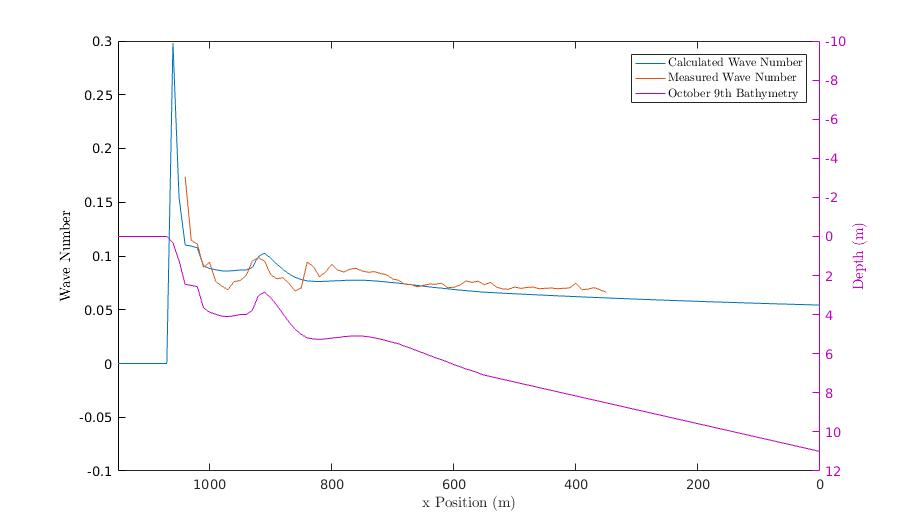
\includegraphics[scale=0.46]{img/Real_vs_Calcd_wavenum.jpg} 
\caption{Noise in Measured Wave Number}
\label{effectivewavenumbernoise}
\end{figure}